\documentclass[12pt]{beamer}
\usepackage{beamerthemeHannover, graphicx, clrscode, amsmath, amssymb, multicol}
\usepackage{verbatim}
\setbeamercolor{sidebar}{use=structure,bg=gray!60!green}
\title{Introduction To Perl 6 Modules}
\author[Duke Leto]{Jonathan "Duke" Leto}
\date{}

\begin{document}

\frame{
    \titlepage
    \begin{center}
        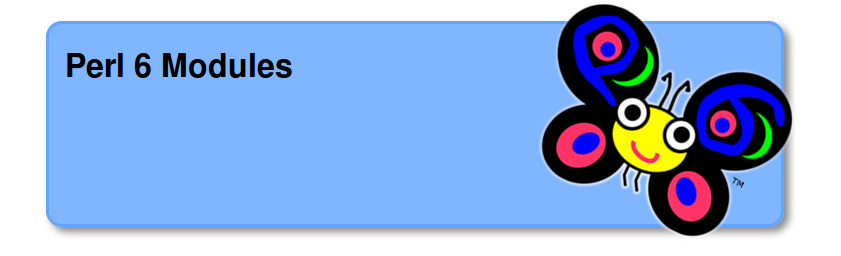
\includegraphics[scale=0.3]{perl6modules}
    \end{center}
}


\section{What is Perl 6?}
\frame{
    \frametitle{Flavors of Perl 6}
    \begin{center}
        \begin{itemize}
            \item Rakudo - Perl 6 on Parrot Virtual Machine
            \item Niecza - Perl 6 on Mono
            \item Perlito
            \item SMOP - C+DSLs
            \item Elf - Ruby
            \item STD.pm - Larry's Implementation in Perl 6 (gimme5)
            \item v6.pm - Source filter for Perl 5
            \item Pugs - Haskell (composting)
            \item others ...
        \end{itemize}
    \end{center}
}
\frame{
    \frametitle{What are Perl 6 Modules?}
    \begin{center}

    Just like Perl 5 modules, Perl 6 modules are units of distributable and
    useful code.

    The CPAN of Perl 6 is called http://modules.perl6.org

    \end{center}
}

\frame{
    \frametitle{Which flavors of Perl 6 to use?}
    \begin{center}
    Different flavors of Perl 6 have implemented different feature sets.

    Rakudo Perl 6 currently has the largest feature set and the most number of current contributors.
    \end{center}
}

\frame{
    \frametitle{How Do I Start Writing a Perl 6 Module?}
}

\frame{
    \frametitle{Anatomy of a Perl 6 Module}
}

\frame{
    \frametitle{Writing Tests for a Perl 6 Module}
}

\frame{
    \frametitle{Running Tests for a Perl 6 Module}
}

\section{Getting Started}
\frame{
    \frametitle{Getting Involved}
}

\section{ Let's Jump In }
\frame{
    \frametitle{Hack Session}
    Ok, let's do some hacking already.
    \begin{itemize}
        \item Checkout source code (git clone ...)
        \item Build Rakudo
        \item Run the Perl 6 Test Suite (long but fun!)
        \item Submit bugs if any tests fail
        \item Experiment!
    \end{itemize}
}

\frame{
    \frametitle{ Thanks }
    \begin{itemize}
        \item Larry
        \item Eric Wilhelm
        \item Patrick Michaud
        \item The Perl Foundation
        \item Everyone working on Parrot, Rakudo and Perl 6
        \item PDX.pm for listening to my rants
    \end{itemize}
}

\frame{
    \frametitle{ Resources }
    \begin{center}
        \begin{itemize}
           \item http://perl6.org
           \item http://modules.perl6.org
           \item TODO: perl 6 planet
           \item \#perl6 on irc.freenode.net
           \item \#parrot on irc.perl.org
        \end{itemize}
    \end{center}
}
\end{document}
